
\ifx\isEmbedded\undefined

\documentclass[12pt,a4paper]{report}
\usepackage[bottom=2.5cm,left=2.0in,right=2.5cm]{geometry}

% FONT RELATED
\usepackage{times} %Move to times font
\usepackage[labelfont=bf,textfont=it]{caption}

% LINKS, PAGE OF CONTENT, REF AND CROSS-REF, HEADERS/FOOTERS
\usepackage{footmisc}
\usepackage{hyperref}
\usepackage{bookmark}
\usepackage{fancyhdr}
%\usepackage{nameref}

% FIGURES, GRAPHICS, TABLES
\usepackage{graphicx}
\usepackage{parskip}
\usepackage{tocloft}
\usepackage{array}
\renewcommand{\cftfigfont}{Figure }
\renewcommand{\cfttabfont}{Table }
\usepackage{longtable}

%\newlength{\mylen}
%\renewcommand{\cftfigpresnum}{\figurename\enspace}
%\renewcommand{\cftfigaftersnum}{:}
%\settowidth{\mylen}{\cftfigpresnum\cftfigaftersnum}
%\addtolength{\cftfignumwidth}{\mylen}






%\usepackage{subfigure}
\usepackage{wrapfig}
\usepackage{caption}
\usepackage{subcaption}


% COLOURS, TEXT AND FORMATTING
%\usepackage[left=2.0in,right=0.5in]{geometry}

\usepackage{array}
\usepackage{color}
\usepackage{setspace}
\usepackage{longtable}
\usepackage{multirow}


% ADVANCED MATHS, PSEUDO-CODE
\usepackage{amsmath}
\usepackage{amsfonts}
\usepackage{alltt}
%\usepackage{algorithm2e}
\usepackage{algorithmicx}
\usepackage{algorithm}
\usepackage{algpascal}
\usepackage{algc}
\usepackage{algcompatible}
\usepackage{algpseudocode}
\usepackage{linegoal}

% BIBLIOGRAPHY
\usepackage{natbib}
%\usepackage[authoryear]{natbib}
%\usepackage{harvardnat}
\bibpunct{(}{)}{;}{a}{}{,}
%\usepackage{bibentry}
%\nobibliography*



% LINE NUMBERS
%\usepackage{lineno}
%\linenumbers

% USE IN DISSERTATION:

% MARGINS
%\setlength{\oddsidemargin}{2.0in}
%\setlength{\evensidemargin}{0.5in}
%\setlength\headsep{2.5in}

% TEXT
\setlength\textheight{9.5in}
\setlength\textwidth{5.1in}

% indent at each new paragraph
\setlength\parindent{1.0cm}
%\setlength\parindent{0.5cm}

%\setlength{\parskip}{10.5ex}

\setlength\topmargin{-0.2in}

% 1.5 spacing:
\renewcommand{\baselinestretch}{1.5}
%\renewcommand{\baselinestretch}{1.3}
%\fontsize{15}{15}\selectfont

% USE IN REPORT:

%\setlength\oddsidemargin{1cm}
%\setlength\evensidemargin{0.3in}
%%\setlength\headsep{2.5in}
%
\setlength\textheight{9.0in}
%\setlength\textwidth{5.5in}
%
%% indent at each new paragrapg
%\setlength\parindent{0.5cm}
%
%%\setlength{\parskip}{10.5ex}
%
%\setlength\topmargin{-0.2in}

%\newcommand{\HRule}{\rule{\linewidth}{0.5mm}}
\newcommand{\HRule}{\rule{\linewidth}{0.0mm}}

% Color definitions (RGB model)
\definecolor{color-comment}{rgb}{0.1, 0.4, 0.1}
\definecolor{color-variable}{rgb}{0.000,0.000,0.616}
\definecolor{color-question}{rgb}{0.4, 0.0, 0.0}
\definecolor{color-new}{rgb}{0.2, 0.4, 0.8}

\newcommand*{\Let}[2]{\State #1 $\gets$
\parbox[t]{\linegoal}{#2\strut}}

\newcommand*{\LongState}[1]{\State
\parbox[t]{\linegoal}{#1\strut}}

\graphicspath{{../images/}}
\begin{document}
%\maketitle
\fi


%**************************************************************************
%**************************************************************************
\chapter{Literature Review}
\label{cha:literature_review}

Clothing as the one of the most distinctive feature of human being that differs us from other creature plays a very important role in our daily live. It can be traced back to 107,000 years ago \cite{Kittler2003} \cite{Toups2011}. The basic function of clothing is to provide protection to the wearer from the elements. It also performs a wide range of cultural and social function. It express the personality, occupation, sexual differentiation and social status of the wearer \cite{Harms1938}.

In the world of today, with its high speed development of computer hardware, realistic virtual character has been wildly used in film production, TV and games. Apart from the character's body and facial expression, same as in reality, costumes play a very important role in acting. For visual realism, techniques have been developed, such as motion capture for animation and muscle system for skin deformation, etc. However, virtual clothing, which involves both textile engineering knowledge and artistic expertise, is still being considered as a challenging and time-consuming work. 

although this topic has been studied for decades, Many techniques have been developed to create the shape of the cloth object and simulate its dynamic behaviours. Most previous work address these two problem in isolation. In the following subsections, several reviews will be made respectively in these areas. Firstly, a general overview of pattern-making in fashion design is presented, followed by the research in anthropometry that explains human body measurements in detail. And then, the state of the art virtual clothing techniques are being introduced. Finally, according to the related research topic covered in this thesis, a brief conclusion of previous research is presented. 


%--------------------------------------------------------------------------
\section{Pattern-making in fashion design}

The creation of a garment is constituted by several interdependent yet inseparable processes. Every each of the process are heavily affects the appearance and fit of the garment. Within these processes, pattern-making settles among the earliest few steps in the creation of a garment. It is a highly skilled craft that bas evolved over the centuries. 

In the ancient Roman period, creating textile was a laborious process. Fabric was weaved using primitive looms entirely by hand. Therefore, Fabric was an very expensive commodity and it was an important symbol for the social status of the wearer. In terms of structure of the cloth at that age, the cloth was mainly consisted by a set of uncut, rectangular shaped fabric pieces to minimize waste \cite{Caroline1996}. 

\begin{figure}[ht]
    \centering
	\includegraphics[width=\columnwidth]{../images/ancient_roman_cloth}\\[1cm]
    \caption{The peplos(left) and the chiton(right) was the common cloth wear by woman in ancient Roman \cite{McManus2003}.}
    \label{figure:fig3}
\end{figure}

In the fifteenth century the seminal art of patternmaking began. The fabric was carefully trimmed to fit the contour to the body \cite{macdonald2009principles}. The foundation of modern fashion design was built since then. Prior to the Industrial Revolution the art of patternmaking was highly revered. Tailors meticulously worked with their client's personal measurements to customize patterns. Clothing made by tailors was elaborate and relegated only to the very rich. With the onset of the Industrial Revolution, standardized patterns were essential to the success of ready-towear clothing. Initial attempts to create standardized patterns resulted in poorly fitting garments with little detail. Men's suits were boxy, plain, ill-fitting sacks. After lengthy experimentation and standardized sizing, patternmaking made a triumphant transformation from customization to standardization \cite{macdonald2009principles}.

%--------------------------------------------------------------------------
\section{Anthropometry}

Fitness is one of the essential factor that directly determines the functionality of the garment. To achieve fit, measurements of the body of the wearer need to be acquired. Anthropometry is the branch of human science that study the measurements of body size, shape, mobility, flexibility and strength. Human body dimension, as ours personality, are largely varied among the population. Many user-centred applications requires the understanding of this variability. Especially for the garment industry, as cloth is an object that its functionality is determined by its coverage and sealability. Both the coverage and the sealability need to be ensured by obtaining wearer's body measurement. This section will debrief the research achievement in anthropometry and introduce the method that acquires the anthropometry data. 

Research of Human physical stature was the first topic in the anthropometry that was studied systematically. The history of it can be traced back into 18th century \cite{tanner_history_1981}. However the recognition of human proportion far earlier than it. 
In ancient Egypt, when paint human figures, a modular grid was employed to the preparation of tome painters drawings \cite{pheasant2006bodyspace}. The modular grid consists of 18 units from the crown of the skull to the foot. This separation provides a consistent point upon which a figure's proportions could be based on. \cite{robins1994proportion} points out that by laying a hypothetical grid over figures from early dynasties it can be demonstrated that their proportions are identical to those of later dynasties.  

\begin{figure}[ht]

    \centering
	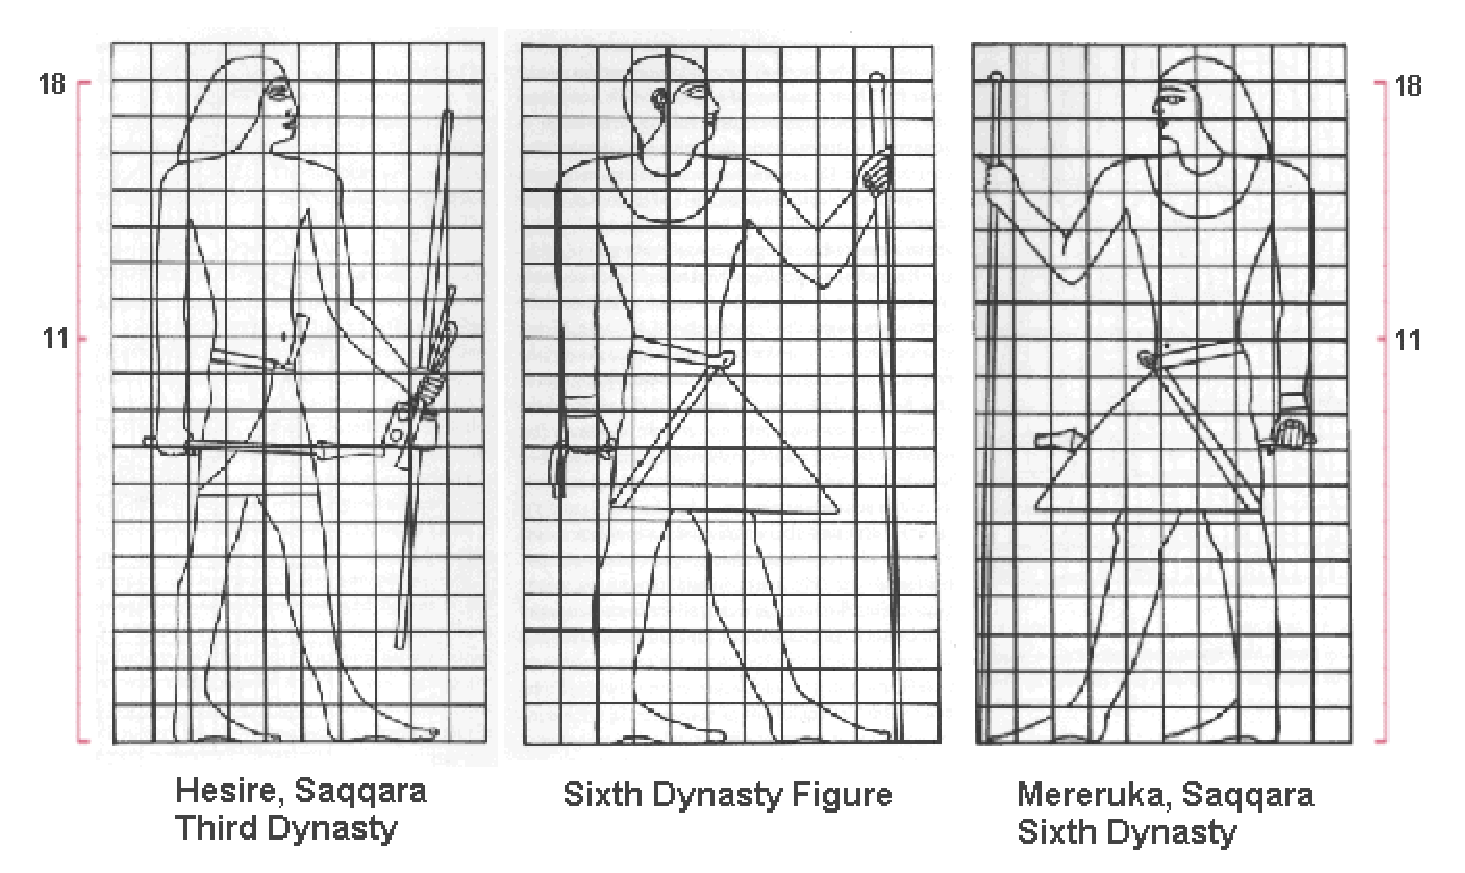
\includegraphics[width=\columnwidth]{../images/threefigures}\\[1cm]
	%
\includegraphics[width=0.3\textwidth]{../images/bu_logo}\\[1cm]
    \caption{The three figures above have a hypothetical grid of 19 squares overlayed 
to show the 18:11 relationship between the height of the hairline and navel \cite{robins1994proportion}.}
    \label{figure:fig1}
\end{figure}

This modular system evolved initially as a drawing standard that still being used today. The most detailed system of human proportions that today's anthropometry researches built on are come from the 15 B.C the Roman architectural theorist Vitruvius \cite{selin2008encyclopaedia}. His theory of human proportions are well known to us as a "well-shaped man" \cite{Rudolf1955}, in which the height of the human stature are equal to its arm span. Vitruvius also employs this human proportion as a fundamental principle in his building design as he claims that "no Temple can have a rational composition without symmetry and proportion, that is, if it has not an exact calculation of members like a well-shaped man" \cite{pollio1914ten, Marcus2002}.

The most recognized Vitruvius's human proportion visualization is the drawing created by Leonardo da Vinci \cite{stemp2006secret}. This piece is accompanied by the nodes that based on the human proportion theory developed by Vitruvius. It depicts a male figure in two superimposed postures that The arms and legs of the male are circumscribed by a cycle and square respectively. When this piece was created, the theory of human proportion had become bound up with the "golden ratio". That is the umbilicus divides the stature of the male person in standing posture in golden section. Such that the ratio of the greater part of the stature to the whole body is equal to that of the lesser part to greater part \cite{stemp2006secret}.

\begin{figure}[ht]
    \centering
	
\includegraphics[width=0.7\columnwidth]{../images/Da_Vinci}\\[1cm]
    \caption{The Vitruvian Man created by Leonardo da Vinci in 1490 \cite{stemp2006secret}}
    \label{figure:fig2}
\end{figure}

However, the study carried out by Vitruvius were based on the Roman population in 15 B.C. In the past two hundred years, anthropometry has shown that span exceeds height in 59-78\% of normal adult white men \cite{Schott19921518}. The study on anthropometry was not systematically carried out until 1870. A Belgian mathematician who named Quetelet published a statistical analysis of the chest sizes of 5000 Scottish soldiers\cite{quetelet2011anthropométrie}. This was the birth of the science of anthropometry. In a very long time after the foundation of this science, anthropometric was mainly used for taxonomic or physiological studies. The developments of this science accelerated during WWII powered by aircraft industry due to the needs to design better aircraft cockpits. Even today, 
much of the anthropometry researches are initiated by military industry. 

The measurements involved in modern anthropometry varies from field to field. In general, 
there are 7 measurements illustrated in the table below:

%\setlength{\tabcolsep}{4pt}
\begin{table}[ht]
        \centering
        %\begin{tabular}{|m{1.1cm}|m{0.8cm}|m{1.2cm}|m{1.2cm}|m{1.2cm}|m{1.2cm}|}
        \begin{tabular}{|l|m{7cm}|l|}
        \hline
        Height & a point-to-point vertical measurement\\
        \hline
        Breadth & a point-to-point horizontal measurement running across the body or segment\\
        \hline
		Depth & a point-to-point horizontal measurement running fore-and-aft along the body\\
		\hline
		Curvature & a point-to-point measurement following a contour\\
		\hline
		Circumference &  a closed measurement that follows a body contour\\
		\hline
		Reach & a point-to-point measurement following the long axis of the arm or leg\\
		\hline
        \end{tabular}
        \caption{The basic anthropometry measurements}
        \label{table:tab4}
\end{table}

Driven by the industrialization of the early nineteenth century, the development of standardization reached to an unpretentiously speed. To largely produce cloth for the general public, the grading system was introduced to the cloth making industry. This is the process that used by clothing manufacturers to produce garments in a range of sizes. Grading is a standard method of applying increases and decreases to make the pattern larger or smaller. 
Generally, there are three steps involved in defining a sizing system \cite{Schofield01012005}: Firstly divide general population into several categories of body types with similar characteristics. Then a body measurement is selected as a primary size interval for each category, finally choose the intervals for remaining body measurements for each category. 

 
%--------------------------------------------------------------------------
\section{Virtual clothing}

Followed by wide use of virtual human in many field, virtual clothing has became a hot research topic that many researches have been done to improve the realism or efficiency of the result. Since there are many processes that involved in a complete reproduction of cloth in virtual world, the computational ability of the hardware is the biggest constrain that limits the quality of the modelling and simulation. When research on virtual human just started, to prevent naked human model, the cloth were usually mimicked by a group of texture that mapped onto the human model. Later, to improve the realism of the cloth, 3D modelled cloth mesh was introduced that cloth are modelled as a part of the character, and the skin that covered by cloth were discarded to reduce the computational requirement. In terms of cloth animation, it directly driven by the same joint system that drives the skin of the character. 

After many years research, today's virtual clothing methods are much different than before. In general, according to the core technique that determines the deformation method of virtual clothing, modern virtual clothing technique can be classified into three categorises: geometric virtual clothing, physical virtual clothing and hybrid virtual clothing. 


\subsection{Geometric Virtual Clothing}

Geometrical method can be traced back to 1986. It was widely used for cloth modelling in the early age. \cite{Weil:1986} presented a  method to generate a hanging cloth using geometrical techniques, the cloth was represented by a grid of vertices and the shape of cloth was generated from catenary curves between the hanging points \ref{figure:weil}, it is not suitable for dynamic simulations but works very well for stationary or single-frame renders. This technique creates an underlying shape out of several hanging points. Then it passes through each set of three of these points and maps a catenary curve to the set. Finally it takes the lowest out of each overlapping set and uses it for the render. This method can only simulate certain shape of damping object and it cannot be used to simulate the whole piece of cloth.

\begin{figure}[ht]
    \centering
	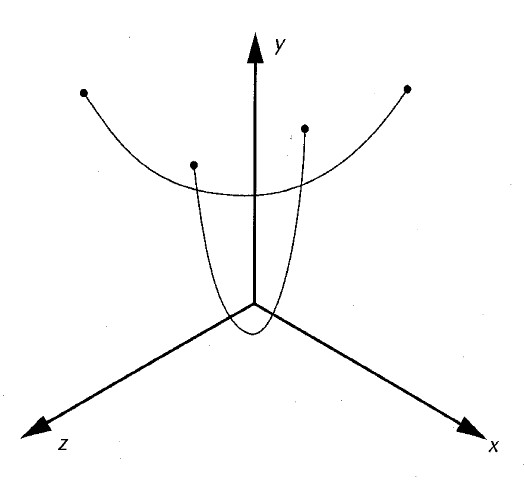
\includegraphics[width=0.7\columnwidth]{../images/weil1986}\\[1cm]
    \caption{Two crossing catenary curves presented in \cite{Weil:1986}}
    \label{figure:weil}
\end{figure}

\cite{agui1990} introduced a method of modelling a sleeve on a bending arm using geometrical algorithm. The cloth is represented by a cylinder surface consisting of a group of circular curves. The wrinkles are created by the consequence of the differences in curvature between the inner and outer part of the sleeve. This method only focused upon the simulating bending sleeve and can only be implemented in the stationary cloth simulation. 

Later on, \cite{Hinds1990} published a series of papers to present the techniques that have the ability to produce the image of an object with cloth covered on very quickly. This method generates the cloth based on the shape of the underlying object layer or skin layer. Those two layers consist of a series of sections and each corresponding section has same number of vertices. The algorithm creates the folds by using gaps between cloth layer and skin layer. Sinusoidal functions are mapped along the fold line to simulate natural folds where cloth is slack. This technique is very fast since it only uses a few simple equations solving the problem. Their methods are used in the interactive garment design but because it cannot generate the motion of the cloth object, it cannot be used in the animation field.

\cite{Miller:1991} presents a novel method named Geometrically Deformed Model. This method is developed for extracting a topologically closed geometric model from a volume data set. This method introduced a simple geometry as an initial object which is already topologically closed. Then based on a set of constraints, this simple object is deformed to fit the object within a volume. At the same time, the deformed object maintains its closed and non-self-intersect.  The major advantage of this method is that the sampled data are aggregated by placing geometrical relationship on the model. This allows a initial convex model to be transformed into a concave object. Since the computational cost are associate with number of the constrain that requires during the deformation, the level of detail can be easily contorted. Later, \cite{Thomas2008} extend this method into cloth simulation. In their method, the cloth mesh are partitioned into triangular clusters. Using these triangular clusters, the optimal rotation can be calculated efficiently for the shape matching presented in \cite{Miller:1991} without iterative calculation for polar decomposition. This method advanced itself with high efficiency, according to the experiment section in this paper, the computation time reached linear time complexity in terms of number of the mesh vertices. 


\cite{DJWBSC06} presents a geometric method for modelling the cloth by warp the developable surface around the character's body in a natural manner to create the visually realistic wrinkle. By flattening the developable surface, this method can also provide the distortion-free sewing patterns for real industry use. In this method, the first step is to use a sketch based interface to generate an initial 2D surface from the contour of the cloth drawn by the user. Then by using distance field technique, the surface is converted into a 3D surface. After that, the seam line is added directly by hand and drawn on the surface. Each surface panel is enclosed by seams while all the panels are kept assembled along the seam line. For the wrinkle handling, in this paper, the wrinkles are categorized into two types, diamond wrinkle which caused by axial compression and aligned wrinkle which caused by twisting \ref{figure:decaudin}. They assumed all the wrinkles occurring on the cloth are different combination of these two types of wrinkles. A procedure buckling patterns is developed to create the natural shape for the wrinkles on the cloth. However, limited by using developable surface to recreate the wrinkles and the numbers of the wrinkle pattern, it can only produce rough shape of wrinkles, which means it cannot reproduce the wrinkle with fine details on it. Moreover, to create a huge variety of wrinkle pattern requires significant large amount of parameter, which will leads to a very heavy computation.  


\begin{figure}[ht]
    \centering
	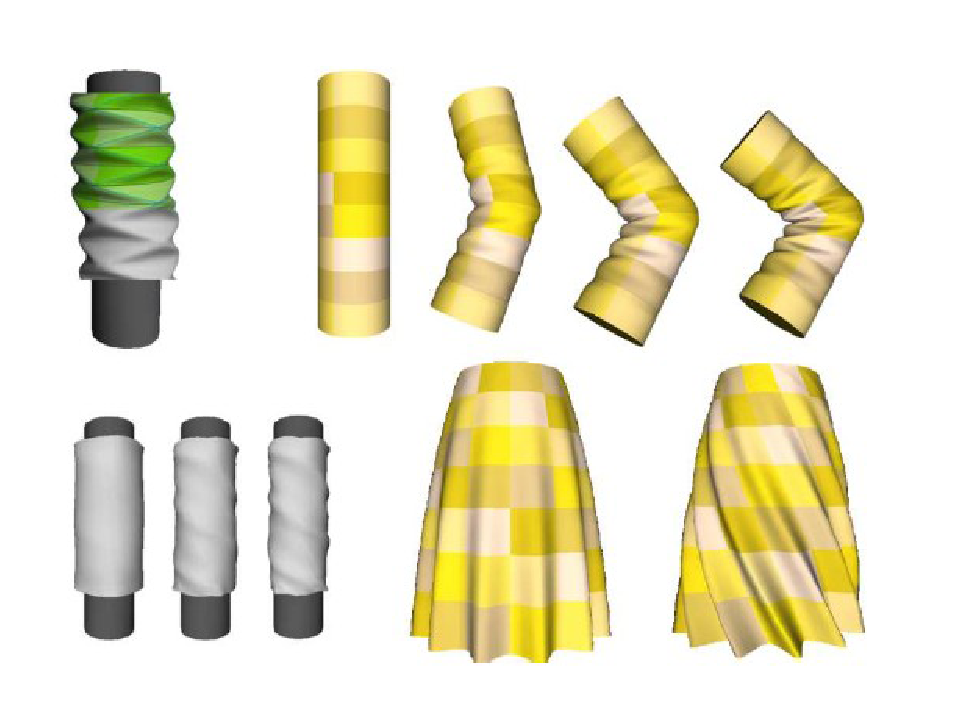
\includegraphics[width=0.7\columnwidth]{../images/decaudin}\\[1cm]
    \caption{Two wrinkle pattern presented in \cite{DJWBSC06}. First row demonstrates the  diamond wrinkle pattern and its derivative. The second row is the aligned wrinkle and its derivative.}
    \label{figure:decaudin}
\end{figure}


\cite{Muller:2010} introduced a geometrical approach to add fine detailed winkles onto dynamic simulated mesh such as cloth or skin. The approach presented uses a higher resolution wrinkle mesh as a reference which attaches to the lower resolution mesh \ref{figure:Muller2010}. The low resolution mesh is composed of the index of its triangle and a pair of barycentric  coordinates that defines a point in the base triangle.  This allows the wrinkle vertices on lower resolution mesh to deviate from their attachment positions within a limited range. The method presented in \cite{Muller:2004} is used for wrinkle generation. The edge splitting method is used iteratively to base coarse mesh till the longest edge falls below a given threshold.

\begin{figure}[ht]
    \centering
	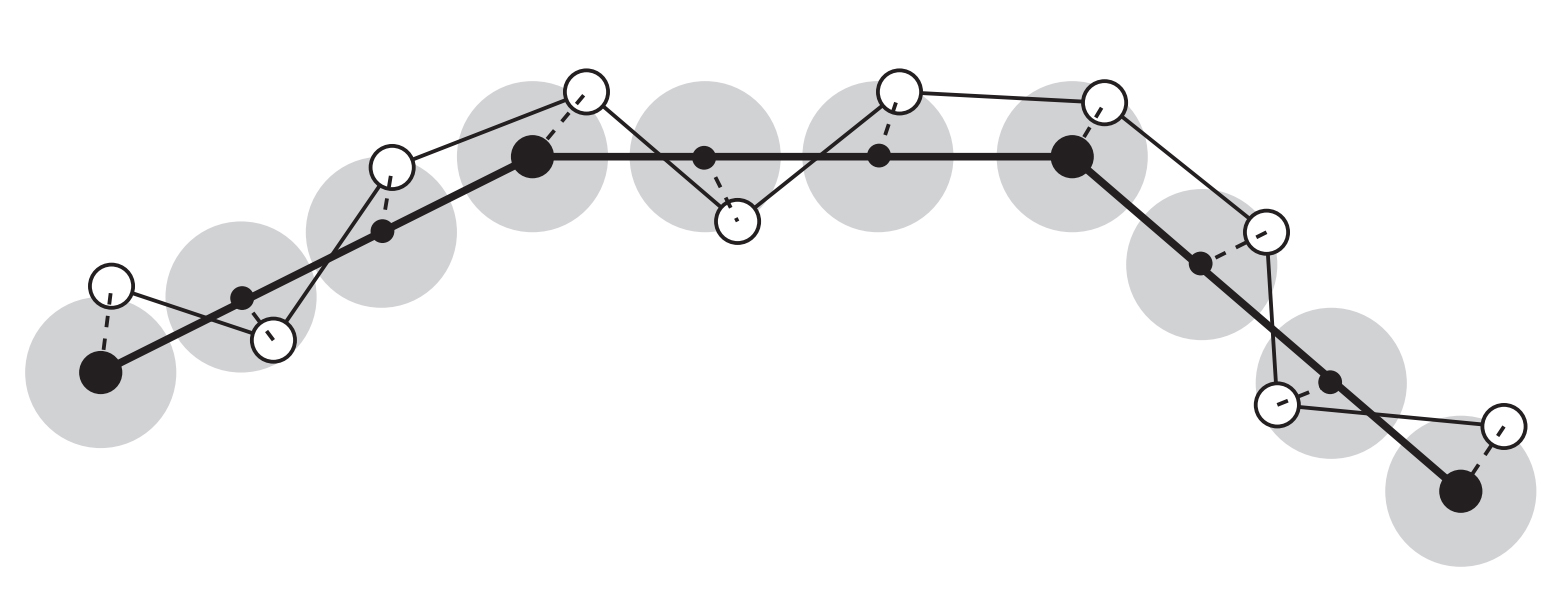
\includegraphics[width=0.7\columnwidth]{../images/Muller2010}\\[1cm]
    \caption{The black dots and thick lines are the vertices and edges of the low resolution base mesh, the white dots and thin lines represents high resolution winkle mesh. The grey region is the constrain area for controlling the movement of white vertex \cite{Muller:2010}}
    \label{figure:Muller2010}
\end{figure}


\cite{Chen:2010} introduced a method for simulating inextensible cloth using fully geometric approach that is subjected to a conservative force (e.g., the gravity) and collision-free requirement. The paper points out that for a piece of cloth, its stretch  resistance and compression resistance are many times larger than its bend resistance. Therefore, the simulated cloth can be considered as an inextensible object. However, traditional physically-based cloth algorithm cannot preform correctly if some of the stiffness coefficients are set to infinite. Thus they provide a method such that the physical-based simulation process is transferred into a deformation process of an initial developable mesh surface to a final mesh surface. The method introduced in this paper is an iterative process that based on energy minimization. Gauss-Newton iteration is used for the minimization of the energy function. However, this method can only handles the conservative force, it cannot handles non-conservative force such as friction. The other crux is that since its uses energy minimization to determine the final shape of the cloth object, the simulated cloth object can only achieve to one steady states therefore it is not suitable for dynamic use. 

\begin{figure}[ht]
    \centering
	
\includegraphics[width=0.7\columnwidth]{../images/chen2010}\\[1cm]
    \caption{blue points are the dynamic anchor points, (a), (b), and (d) are three intermediate states in sequence. Although collision occurs the number of dynamic anchor points are reduced gradually; (c) and (e) are the two sequent intermediate states where the potential energy of the mesh is lowered gradually. (f) is the final state where the potential energy reach to the minimum \cite{Muller:2010}}
    \label{figure:chen2010}
\end{figure}

Geometrical cloth modelling method may fast on generating the static cloth shape. But cloth is a soft object whose shape is closely associated with the shape of body underneath. In addition, when it comes to the detail of the wrinkle, the number of the perimeters needed to create it will increase dramatically then lead to a heavy computation.  However, physics can generate the detail wrinkle easily and can also reproduce the kinetics property of textile very well.

\subsection{Physical Virtual Clothing}
Physical method represents the cloth using a set of particles connected to each other by springs which can replicate the behaviour of the soft flexible object such as textile. The number of neighbourhood particles varies according to the different technique it uses. Generally, there are two kinds of model for the physical cloth modelling technique, Energy-based techniques and the Force-based techniques. Energy-based model calculate the total energy of the cloth using a set of energy equations.
 
Those equations determine the shape of the cloth by moving the vertexes (particles) to achieve a minimum energy state. This kind of methods is widely used in static simulations. Because the energy model is based on the kinematic theory in which the shapes are compositions of geometrically or algebraically defined primitives. And it does not interact with each other or with external forces. By this reason, the Force-based technique has been brought in to this field to describe the reaction to external forces. It usually uses differential equation to represent the force among each vertex and perform a numerical integration to locate vertex position at each time step. This kind of methods is used in dynamic simulations. 


\cite{Terzopoulos1987} introduced a method using the physically-based model to construct the shape of a cloth object. Their method is based on the elasticity theory used to represent the shape and motion of deformable materials, and moreover has the ability to be interactive with other physically-based models. The simulation model introduced in this paper is based on the simplifications of elasticity theory to deformable curves, surfaces, and solid objects. It has the ability to generate static shapes by simulating their physical properties such as tension and rigidity fig.\ref{figure:Terzopoulos1987}. Moreover, by bring the physical properties such as mass and damping in to simulation, it can simulates the dynamic of these objects. \textit{"The simulation involves numerically solving the partial differential equation, govern the evolving shape of the deformable object and its motion through space."} \cite{Terzopoulos1987} However, this method can only simulate interaction between simple shaped objects, it does not have the ability to simulate cloth wearing by the character.


\begin{equation}
\sum(Particle{i,j}) = K{s}E{s,i,j} + K{b}E{b,i,j} + K{g}E{g,i,j}
\label{equation:eq1} 
\end{equation}

Where $K{s}$, $K{b}$ and $K{g}$ are elasticity, bending and density constants. The total energy E includes elasticity energy $E{s}$ , bending energy $E{b}$ and gravitational potential energy $E{g}$.


\begin{figure}[ht]
    \centering
	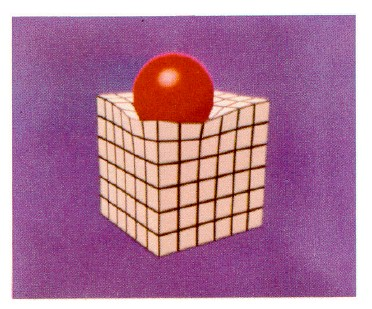
\includegraphics[width=0.7\columnwidth]{../images/Terzopoulos1987}\\[1cm]
    \caption{The simulation result generated in \cite{Terzopoulos1987} by minimizing equation \eqref{equation:eq1}}
    \label{figure:Terzopoulos1987}
\end{figure}


\cite{Volino2005} introduced a general mechanical model for cloth simulation.  This model uses a accurate particle system model for dynamic simulation instead of mass-spring system because the mass-spring system cannot represents the anisotropic nonlinear mechanical behaviour of textile object. By defining three main mechanical properties of cloth: weft and warp elongation and shear, a triangle face of cloth mesh is described by three 2D coordinates correspond to these three properties. Those three coordinates describes the location of the triangle's vertices on the weft-warp coordinate system that defined by the directions U and V with an arbitrary origin fig. \ref{figure:Volino2005}. This particle system model is able to simulate the anisotropic nonlinear mechanical behaviour of a cloth object using polynomial spline approximations of the strain-stress curves. Furthermore, the aforementioned three mechanical properties can be measured from real cloth piece using Kawabata Evaluation System (KES) of the SiroFAST method. Since the high accuracy their system is able to produce, it suits the requirements of garment design and textile engineering.


\begin{figure}[ht]
    \centering
	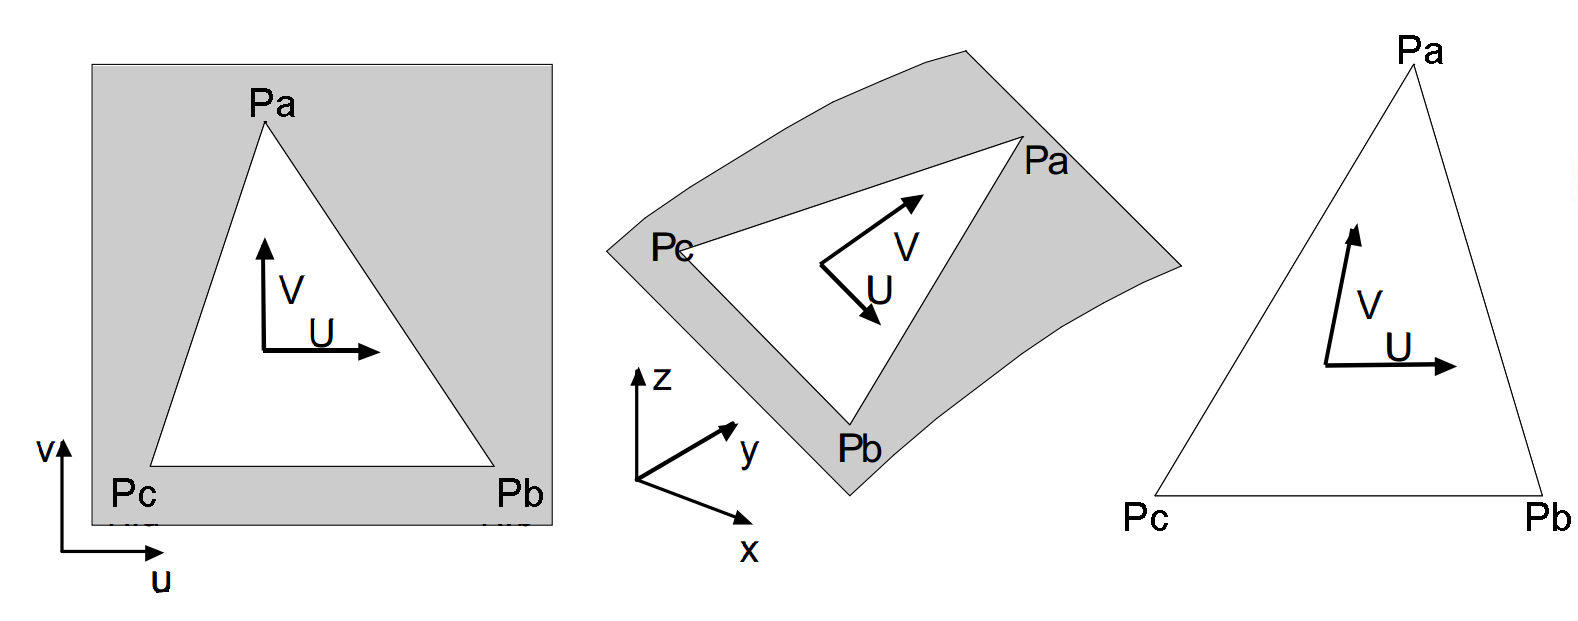
\includegraphics[width=0.7\columnwidth]{../images/Volino2005}\\[1cm]
    \caption{(left) A triangle face of cloth surface defined on the 2D cloth surface. (middle) The deformed triangle in 3D space. (right) The deformation of the weft-warp coordinate system of this triangle face.}
    \label{figure:Volino2005}
\end{figure}


\cite{Volino2009} proposed a simulation model for large deformations of textile. It can reproduce the nonlinear tensile behaviour of textile with accuracy and robustness. Meanwhile the process of simulation remains simple and which is suitable for high-performance simulation system. Differing from the majority of existing cloth simulation systems, with this model, the weft, warp and shear tensile behaviour usually considered in the traditional textile engineering are represented by accurate strain-stress curves.  This model also includes the elasticity and viscosity which makes it suitable for dynamic motion simulation. Most importantly, the computation involved in this method is not much more than mass-spring model but offers a significantly more accurate result.
The technique proposed in this paper has already been implemented into a virtual prototyping system which allows the simulation of accurate mechanical properties of complex garments. 


\cite{Kaldor2010} presented a method which particularly focused on the yarn-based cloth simulation. Yarn-based cloth simulation differs from sheet-based cloth simulation which is wildly used in animation. For the Yarn-based cloth simulation, it always needs enough detail to describe the shape of yarn which leads to an expensive compute. In this paper, a method is proposed for approximating penalty-based contact forces in yarn-yarn collisions by computing the exact contact response at one time step. After that, they use a rotated linear force model to calculate forces in nearby deformation. Their method can speed up contact force by breaking it up into a group of disjoint regions and adaptively constructing local models for each region to approximate the true force response. This method only targeting on the yarn-based cloth simulation, it cannot handle other types of cloth simulation.


Physical method calculates the inter-force amongst each vertex. The number of vertex which construct the cloth directly influences the apparelling of the simulation. To produce a fine detail result the mesh resolution for cloth must stay high which leads to a very heavy calculation. Thus it has been mainly used in off-line high accrue simulation such as garment industry and off-line film production. 

\subsection{Hybrid Virtual Clothing}

Hybrid method combines physical and geometrical and many other methods together to produce a fine result meanwhile minimize the calculation. 

Rudomin (1990) represents a method uses geometrical approximation to reduce the computation time which required by physical techniques. In his method, firstly, the convex hull is constructed by wrapping the object in the cloth. Then the bottom of the convex hull is removed and a point is created along the line of the object’s centre of mass. After that, the point is added in to the convex hull to rebuild it. In the next step, he developed an algorithm to map the upper hull onto the cloth object and removed all the points which lie outside the hull. Then the points which stay inside the hull are used to construct the mesh to give the shape of the draped cloth. After that, the Terzopoulos deformable model (Terzopoulos et al. 1987) is used to refine the mesh of the cloth. His method is only able to simulate the sleeve on a bending arm. 

Kunii  (1990) points out that when using the physical method to model the cloth, the textile are usually represented by many small elements, the polygons, the more detail required the more computation time is. Moreover, the differential equation which represents the cloth object is difficult to obtain the right parameters. This paper also indicates the limitation of the geometrical cloth modelling technique. Therefore, a hybrid method is proposed in this paper to overcome the drawback of both methods. Firstly, physical method has been used to simulate the sewing process which a piece of cloth can be encircled to the body, for example the sleeves which warped around the arms. The grid with springs connected in-between each others are used to represent the cloth object. During this process two kinds of energy are defined, metric energy and curvature energy. The shape of the cloth object is determined by the energy minima using the gradient descent method. In the next step, the wrinkles are refined by using the singularity theory. Then the wrinkles continue to be simulated using the features which includes position of the feature points and the contours of the wrinkles captured from real cloth. Although his method simplified the physical method by integrate the geometrical modelling techniques, it still has many limitations such as the feature points which corresponding to the data captured from real cloth should remain constant. Moreover, the contours become sharper and the wrinkles become deeper after animation.

Tsopelas  (1991) introduced a hybrid technique to generate folds on the cloth without collision in-between itself or between underlying bodies. The cloth is represented by the cylinder under the axial loads and the folds on the cloth are simulated by using thin-walled deformation theory. This process focuses on the area where the folds most likely occur, such as back of the knee, elbow or around the seams where the regions has large curvatures. Once the loads add onto the cylinder, diamond shape patterns occur. After the diamond shape patterns have been located, the algorithm traces several principle curves in each pattern and fit them with elastica. Then the deformation of each elastica is calculated. The non-uniform B-splines is used to interpolate between the points on the elastica to construct the deformed surface. When apply to animation, new principle curves are traced and elasticas are fitted for each step. This techniques was implemented on SUN Sparc2 workstation.

Sunil et al. (1999) introduced a geometric and texture based method to cloth wrinkle generation. Wrinkles are generated from the bump map on a coarse physical simulation of the cloth object and the bump map is created by user. Then the wrinkles are animated by modulating as per cloth deformation. Based on the theory of cloth having very little in-plane deformation and most of the deformation comes from buckling, using the length changing of the triangle edge to determine the depth of the bump map can simulate wrinkle efficiently. However, the direction of the wrinkle on the bump map has to significantly differ such as the wrinkle of the same location on the cloth in two different bump is perpendicular to each other. Thus there can be a limited number of bump maps created and the variety of the wrinkle is consequently limited.

Lawrence et al. (2005) introduced a kinematic method for generating wrinkles on cloth for CG characters by artist. In this method, the wrinkles are created by artists using the curve-based method on different poses. The wrinkle can be created by using any geometric sculpture software then stored into database. After that, based on the stretch distribution of the cloth on different poses, the wrinkles are sorted in to different category corresponds to the poses. During the animation, the cloth is simulated by coarse physical simulation to handle its global deformation. Then by matching the similar stretch distribution of current cloth to the reference pose, the corresponding wrinkle is mapped onto the animated cloth. Because the wrinkle generated by pure physical simulation is not what the artist wants. By using this method, all the wrinkles are sculpted by the artists, giving them more control ability. Moreover, by setting up the wrinkle database, wrinkles can be easily transferred in to a different character, which improve the production efficiency further. However, this method was mainly focused on how to create wrinkle on one layer tighter garment. The looser garment still need to be simulated by physical method and the interaction between the tighter cloth and the looser garment is very difficult to handle.

Popa et al. (2009) introduced a method for bringing the fine folds into captured cloth using data-driven dynamic wrinkling. In this method, the shape and the position of the wrinkle are captured from video footage based on the wrinkle’s distinguishing shape characteristics, and then the wrinkles are created by using stretch-minimizing deformation, which produces believable wrinkle shape. However in this method, the detail of the wrinkles captured is bounded from below by mesh resolution. The experiment presented in this paper has already used about 100K mesh for a single cloth during the wrinkle capture. But the results shown in this paper indicate that there is still a significant amount of detail lost during the capture. 

Wang et al. (2010) proposed a technique which combines the synthesized fine wrinkle details with coarse physical simulation to produce high quality cloth wrinkles. In this paper, they point out in some scenarios that mostly focused on the appealing, the highly realistic wrinkle can be mimicked by matching a database of pre-extracted wrinkle configurations. The wrinkle database is constructed by pre-simulate its dynamic behavior using high resolution physical simulation. After that, the global dynamic behavior of the cloth can be generated by coarse physical simulation on low resolution mesh meanwhile the motion of the joint responsible for the certain area of skin deformation is also recorded. Although the pre-simulation is highly time-consuming, once it has been done, it can be used for a wide range of motions. In the next step, for each joint certain mesh template is used to create the individual wrinkle for certain motion. Then all the joint wrinkles are merged together into a fine mesh for the cloth simulation. Finally, the low-resolution mesh is simulated using physical method to calculate the collision, gravity, and many other interactions between the character’s body and the environment.


Feng et al. (2010) introduced a hybrid method which can provide high-quality dynamic folds and wrinkle for cloth simulation while still maintaining real-time ability. This method captures the relationship between the two different resolutions of mesh by using data-driven model. Then this relationship is used to transforming the lower quality deformation of the lower resolution mesh through a mid-scale deformation transformation onto the higher resolution mesh with the fine details added on. In the animation pipeline which they developed, during each time step, it starts with the physical simulation for the low-resolution mesh. After that, the deformation transformation and collision detection is executed. In this step, two stages of nonlinear mapping are used to generate the deformation of high-resolution mesh. At the first stage, the deformation for the mesh with the lowest resolution is mapped onto a mid-resolution object which using proxy bone to represents a local region on the high-resolution cloth object, and then the deformation of the proxy bones are mapped onto the high resolution to create the final fine-scale deformation.   Collision detection is also a critical and time-consuming process during cloth simulation. In this paper, they proposed a method of using the proxy bones originally for the mid-scale cloth deformation to represents the high-resolution cloth object to interact with the model of character. The bounding volume is attached to every proxy bone which represents a small area on the cloth object. When the character moves, instead of calculating the collision between each mesh triangles of the cloth and body model, they can calculate the collision between each proxy bone. Although the accuracy of collision handing is slightly reduced, the computation time for the collision test are reduced significantly. Although the efficiency has been improved significantly, like other data-driven method, it requires a time consuming pre-simulation to gain the training data. Moreover this method cannot handle the self-collision of cloth.

Nowadays, virtual clothing has had to rely heavily on physically-simulated cloth in the production environment. The physical cloth simulation system can produce visually realistic results and have become widespread used in the production. But the computation cost of the physical method is still very high, especially with hundreds of characters in the same scene.  The hybrid method combines with different kind of technique into one package to solve the problems in cloth simulation. Those techniques which has been combined with can overcome the drawbacks of pure physical simulation to provide a more effective and efficient solution for the virtual clothing. Especially in those areas which focus on the visual result more than the physical accuracy.    

\subsection{Summary}

In this chapter, a brief history of cloth simulation in computer graphic has been reviewed.  
In general, there are three kinds of techniques to modelling and simulating the cloth. 
The geometrical method is the fastest way to generate the cloth but it does not consider the physical properties of cloth. It represents the cloth by geometrical equations. For that reason, normally it is used as a modelling tool for cloth design in static situations. And it needs a considerable amount of direct user operation to create a cloth. 

The physical method describes the cloth as a dynamic model which changes its shape by time or forces. The shape of cloth is determined by the forces or energies of vertexes. This method not only be able to model the cloth for static simulation but also has the ability to be applied in dynamic simulation. It has already being widely used in garment industry and animation. As the number of the elements which represents the cloth directly determines the detail of the simulation, therefore it is a heavy computation method to produce fine detail result.   

The detail of the apparelling for the simulation done by physical method is directly determined by the quantity of basic element it uses such as polygon or particle. For this reason, the only way to increase the detail level of the simulation is to increase the resolution of the mesh or particles. This directly leads to the incensement of the computation. Especially with the high speed of development of film production, TV, games and online trading, more and more applications require real-time ability of cloth simulation or seeking for a new method that in order to speed up the current simulation procedure. Thus, the hybrid method is bringing into the cloth simulation area. Based on the geometrical method or physical method, combine with other computer techniques such as, data driven method, image based modeling, etc. the most time consuming task which is fine detail wrinkle generation is usually handled to other high efficiency methods rather than physical calculation. Thus, the hybrid method has the ability to overcome many drawback of each method on its own and provides a high efficiency approach to the application. 
However, the hybrid method also has its own drawbacks, because it using other techniques such as data-driven to simulate the wrinkle instead of producing them by solving the physical equation. It is very complicated to handle the complex interaction in-between the cloth and environment such as the self-collision. Moreover, due to bypass the physical model solve the fine wrinkle generation which actually caused by complex stress applied on the cloth, to reproduce realistic wrinkle requires a large number of training data or a complex empirical model. The work load of pre-production is increased heavily. Thus, to design a method which models based on the measurements to fit the character whilst in the meantime using data-driven technique to generate the fine wrinkle instead of using high accuracy physical simulation to speed up the simulation of the virtual clothing is the major research problem of this research.



%**************************************************************************
%**************************************************************************


\ifx\isEmbedded\undefined
% References
\addcontentsline{toc}{chapter}{References}
\bibliographystyle{../ref/harvard}
\bibliography{../ref/phd_references}
\pagebreak
\end{document}
\fi
